% To create a slide, use the following:
% \begin{frame}{TITLE}
%     BODY
% \end{frame}


\begin{frame}{Getting Wave Displacement}
    \centering
    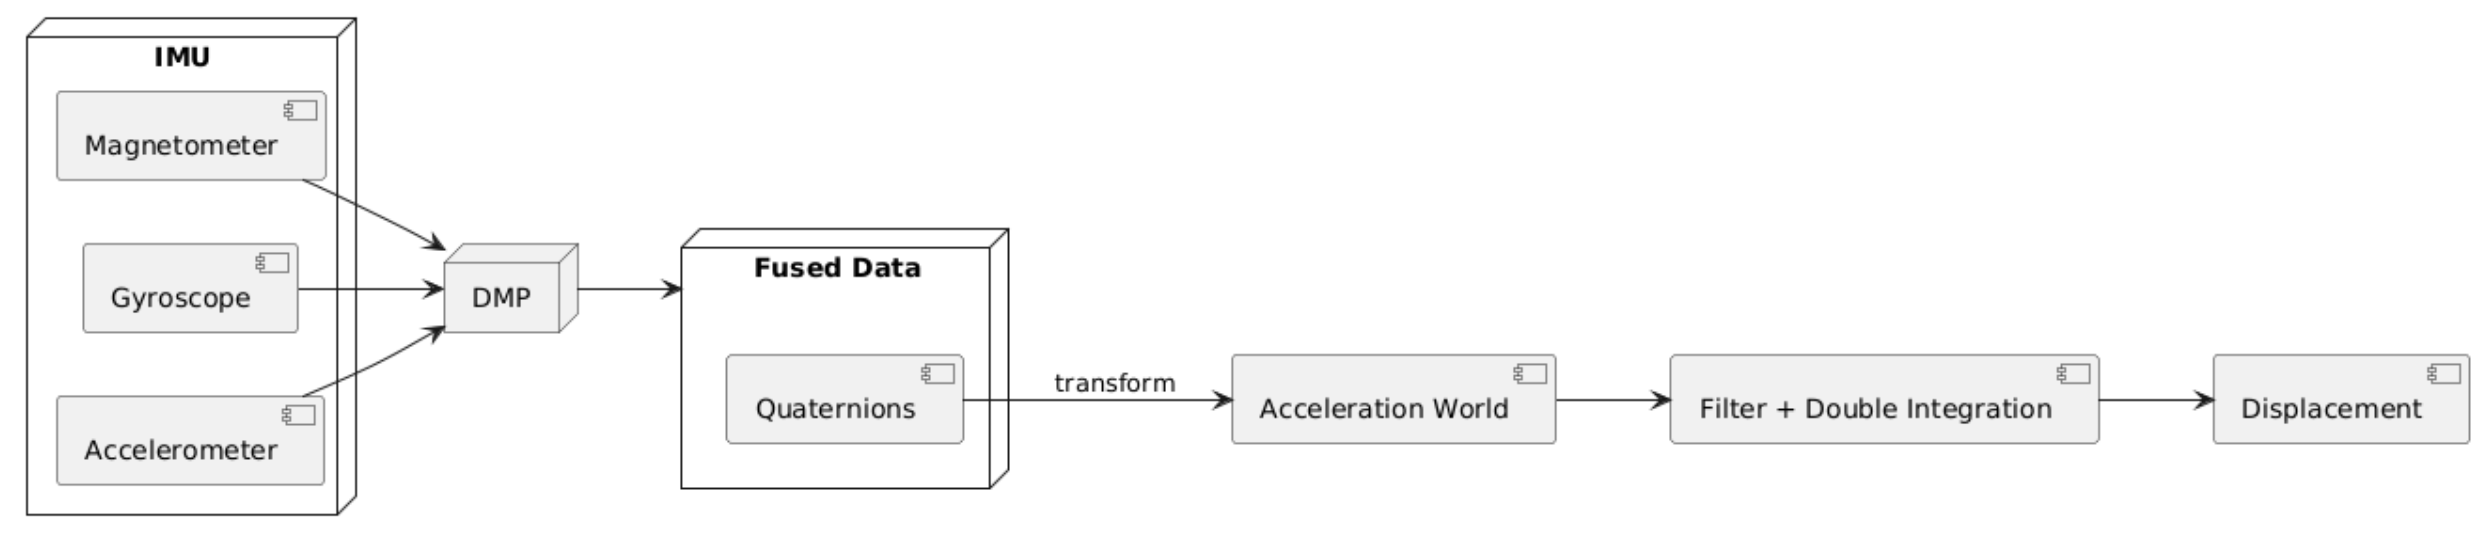
\includegraphics[height=1\textheight,width=1\textwidth,keepaspectratio]{images/wavedisp2.png}
\end{frame}

\begin{frame}{Testing PCBv3}
    \centering
    \includegraphics[height=0.5\textheight,width=0.5\textwidth,keepaspectratio]{images/pcbv3.png}
\end{frame}

% To create a slide with numbered list, use the following:
% \begin{frame}{TITLE}
%     \begin{enumerate}
%         \item ITEM 1
%         \item ITEM 2
%     \end{enumerate}
% \end{frame}

% To create a slide with a graphic:
% 1. Add the graphic to this folder (named picture.png)
% 2. Use the following:
% \begin{frame}{TITLE}
%     \centering
%     \includegraphics[height=0.7\textheight,width=0.7\textwidth,keepaspectratio]{picture.png}
% \end{frame}

% To create a slide with two columns, use the following:
% \begin{frame}{TITLE}
%     \begin{columns}
%         \begin{column}{0.5\textwidth}
%             COLUMN 1 BODY
%         \end{column}
%         \begin{column}{0.5\textwidth}
%             COLUMN 2 BODY
%         \end{column}
%     \end{columns}
% \end{frame}
